\section{Jiongcheng Luo (Roger)}
\subsection{Purpose}
The traditional methodology for an airplane Head-UP Display (HUD) to provide flight information is by obtaining data from a mounted device call Inertial Reference Unit on the aircraft. This method outputs precise and aligned data to the HUD through a mechanical alignment system. Yet, the industrial production of this mechanical alignment system is time consuming and costly. In addition, the current system does not compensate for airframe droop during flight. The purpose of this project is to develop a demonstration system to prove that there is such an algorithm or mathematical procedure that can generate precise and aligned data with reduced installation cost utilizing the data from multiple inexpensive IMUs. This algorithm can handle multiple groups of data in near real-time and the outcome (aligned-data) of this algorithm will compensate the alignment error correctly, and the alignment error should be within a range of one milli-radian.

\subsection{Current Stage}
Currently, we have completed the hardware setup that using a Metro Mini microcontroller and MPU-9250 IMU, the microcontroller and IMU are hooked up by using I2C protocol, and we can now use Arduino IDE for programming. From the perspective of software, we are able to recognize the address of connected IMU and read the output data from all three sensors of the MPU-9250 including acceleration (accelerator value), gyroscope values and magnetometer value. 
In addition, we discovered two different filtering algorithms for getting quaternion output based on the raw data of the sensor, which we can generate quaternion value by using sample code and existing libraries. 

\subsection{Remaining work}
\begin{itemize}
	\item Add multiple IMUs onto single microcontroller. We still need to figure out how to connect slave IMUs and select the correct address of expected IMU by using I2C protocol. 
	\item Get precise error of all IMUs/ sensors
	\item Develop an alignment algorithm for aligning a group of quaternion data.
	\item Develop demonstration interface.
\end{itemize}

\subsection{Problems and Solutions}
\begin{itemize}
	\item \textbf{Problem 1:}
	Knowing the actual error of the IMU/sensors. It is difficult to measure actual precise error of the sensor data by just looking at it output data since the error could be very minor and unstable.\\

	\textbf{Solution:}
	A solution to measure the error is by comparing the actual alter angle with the sensor output data. An actual alter angle can be calculated by using a laser pointer and a mechanical angle adjuster as figure~\ref{fig:widget} for assistant tool, as well as applying trigonometric algorithm. Look at experimental design description for more detail.\\

	\item \textbf{Problem 2:}
	A declination is a factor that would cause error to the yaw data in different region on the earth, the declination needs to be counteract before getting the real yaw data.\\

	\textbf{Solution:}
	A simple solution is to look up the declination value from NOAA (National Centers for Environmental Information) at this region and time. Adding/subtracting the value (in degree) to the raw yaw data.

\end{itemize}



\subsection{Interesting Code}
\begin{lstlisting}[language=c]
static Quaterniond toQuaternion(double pitch, double roll, double yaw)
{
	Quaterniond q;
	double t0 = cos(yaw * 0.5);
	double t1 = sin(yaw * 0.5);
	double t2 = cos(roll * 0.5);
	double t3 = sin(roll * 0.5);
	double t4 = cos(pitch * 0.5);
	double t5 = sin(pitch * 0.5);

	q.w() = t0 * t2 * t4 + t1 * t3 * t5;
	q.x() = t0 * t3 * t4 - t1 * t2 * t5;
	q.y() = t0 * t2 * t5 + t1 * t3 * t4;
	q.z() = t1 * t2 * t4 - t0 * t3 * t5;
	return q;
}
\end{lstlisting}

This piece of code is using a mathematical algorithm that take the pitch roll yaw data to calculate quaternion. There are also other ways like Madgwick filter algorithm and Mahony fliter algorithm that can generate more precise quaternion values.\\

\subsection{Experimental Design Description}
This is an experimental design for measuring the actual error of the IMU sensor. A method to precisely measure the error is to compare a known inclined angle with the calculated angle from two sensor output results (before and after incline). 

\begin{figure}
	\centering
 		\caption{Mechanical Angle Adjuster}
      	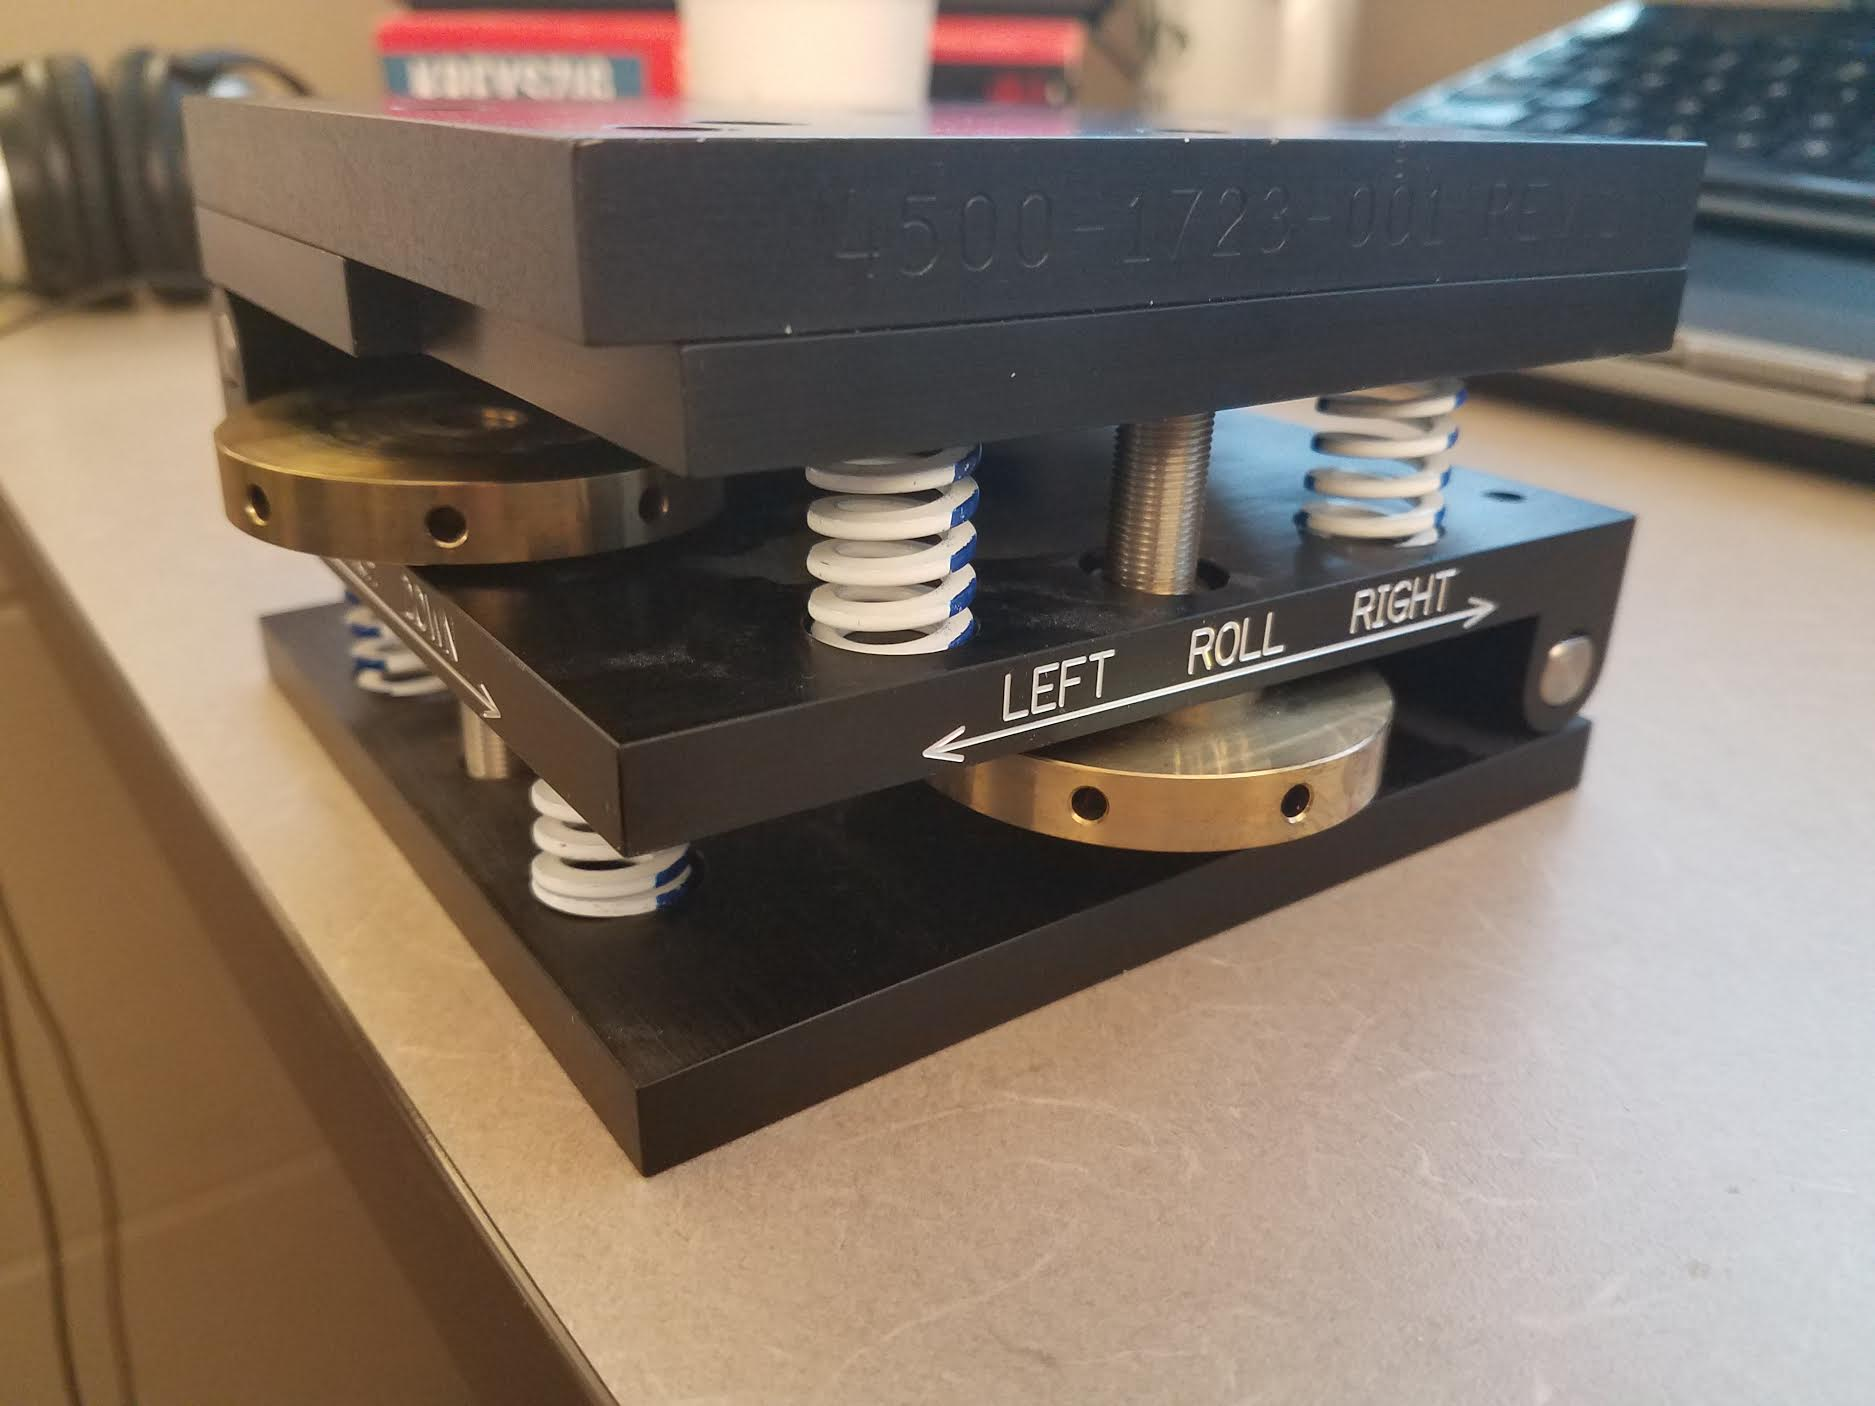
\includegraphics[width=0.8\textwidth,height=0.8\textheight,keepaspectratio]{img/widget}
    \label{fig:widget}
\end{figure}

The experiment will be using a laser pointer and a mechanical angle adjuster as figure~\ref{fig:widget} for assistant tool. A mechanical angle adjuster allows to be manually set for getting a certain degree of angle for simulating yaw, pitch and roll, that will be able to provide a stable motion for the IMU as well as error measurement. A laser pointer is also necessary, that a laser is for constructing a triangle by using the initial distance between the laser pointer and the wall (a), alternative distance between the laser pointer and wall, as well as the distance between two spotlight (b), refer figure~\ref{fig:draft}:

\begin{figure}
	\centering
 		\caption{Draft graph of error measurement experiment}
      	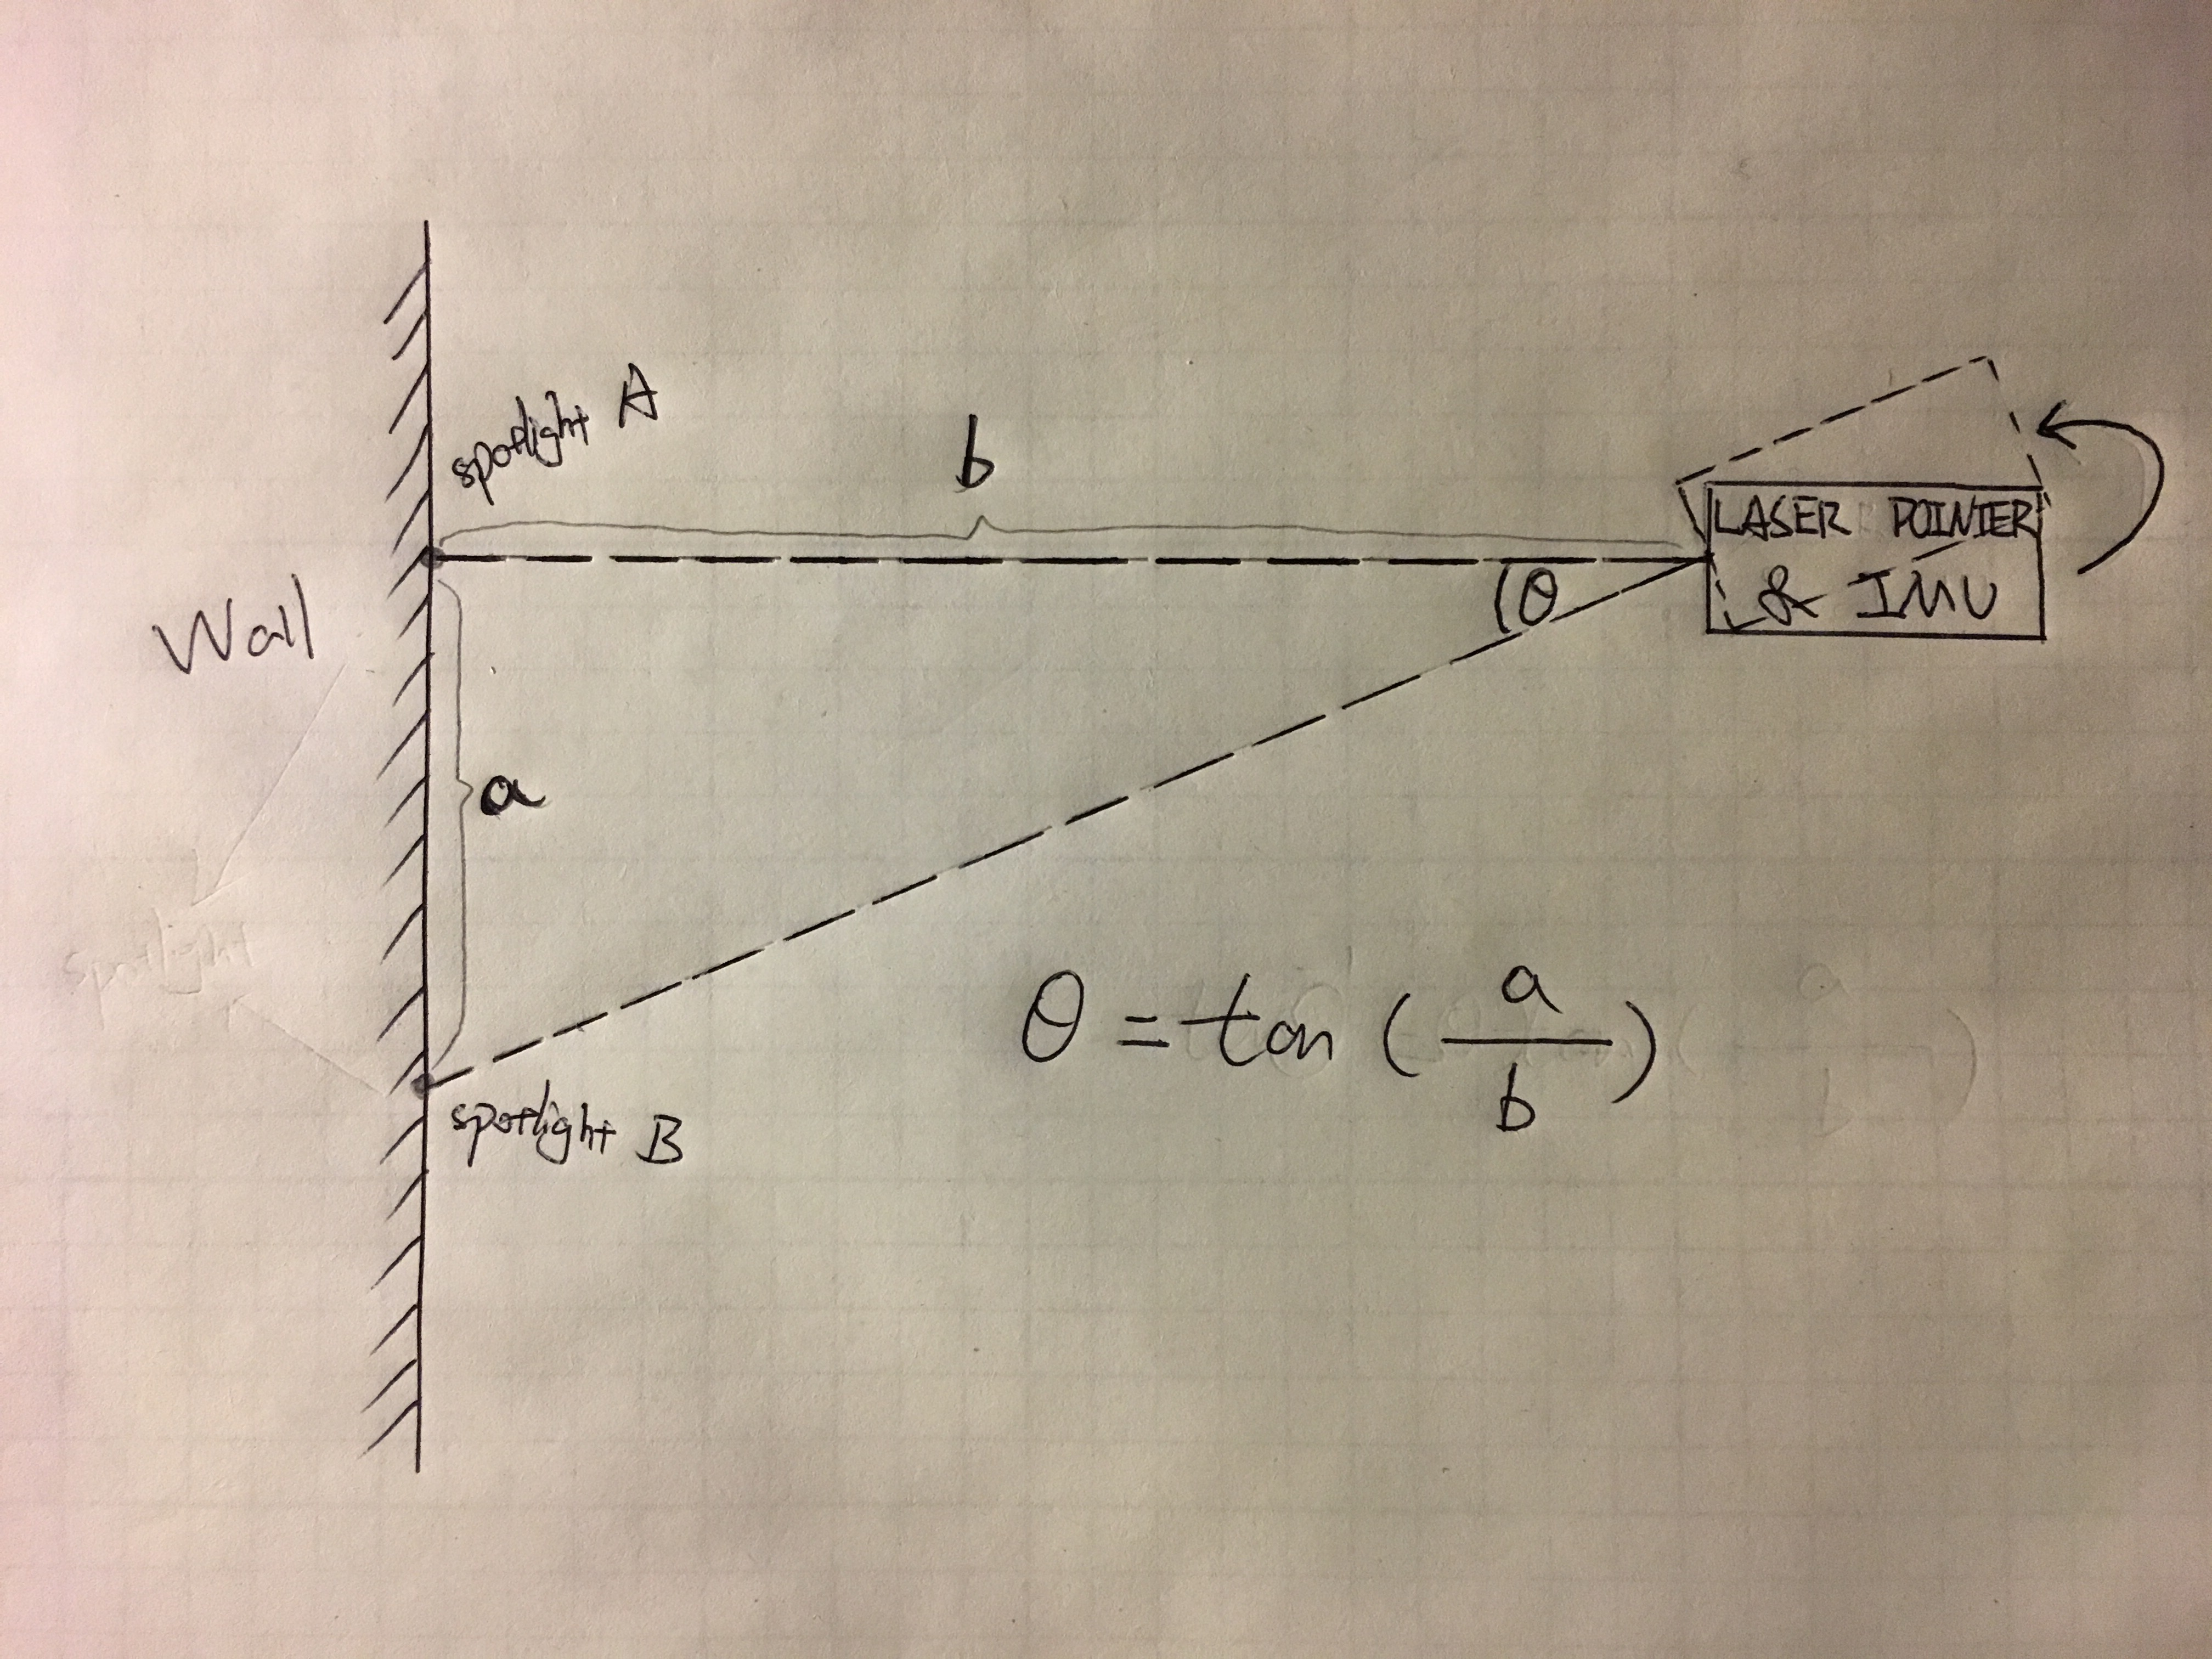
\includegraphics[width=\textwidth,height=\textheight,keepaspectratio]{img/draft}
    \label{fig:draft}
\end{figure}

Theta represents the angle between adjusting the angle, and by measuring the distance value of “a” and “b”, theta can be calculated by applying trigonometric function. Assume theta is the actual precise angle (in radian), the error of the IMU sensor can be measured by comparing the actual precise angle with the output data from the IMU.






